\chapter{Grundlagen von Datenbanken}
\bauer
	\section{Allgemeines zu Datenbanken}
	%Quelle: https://www.oracle.com/de/database/what-is-database/)
	\subsection{Definition}
	Eine Datenbank\footcite{oracle} ist definiert als eine Sammlung von Informationen oder Daten welche im Normalfall auf einem elektronischen Medium wie einer Festplatte abgelegt werden. 
	Der Zugriff auf die Daten erfolgt meist durch ein Verwaltungsprogramm. In den Grundzügen könnten die Daten auch simple Textdateien oder Papiere sein, welche per Hand befüllt und ausgewertet werden. 
	Dies ist allerdings nicht die Norm, denn in der Industrie werden meist Datenbankverwaltungssysteme benutzt welche von einem externen Anbieter zur Verfügung gestellt werden (Oracle, MongoDatabase, Microsoft SQL Server).	
	%Quelle: https://www.mongodb.com/nosql-explained/nosql-vs-sql
	\subsection{Arten von Datenbanken}
	In der Datenverarbeitung wird grundsätzlich zwischen zwei Arten von Datenbanken unterschieden, auf der einen Seite gibt es SQL Datenbank und auf der anderen Seite NoSQL Datenbanken. 
	Einer der größten Unterschiede dieser beiden Datenbanken ist, wie die Daten strukturiert und abgespeichert werden.
	%Quelle: https://de.wikipedia.org/wiki/SQL
	%Quelle: https://www.businessnewsdaily.com/5804-what-is-sql.html#:~:text=%2C%22%20Palic%20said.-,SQL%20history,Data%20Banks%2C%22%20in%201970.
	\subsubsection{SQL (Structured Query Language)} 
	In einer SQL Datenbank werden die Daten durch eine klar definierte Struktur in Tabellen gespeichert und auf der Festplatte abgelegt. 
	Die Structured Query Language, früher bekannt als 'SEQUEL' wurde in den 1970er von Raymond Boyce und Donald Chaberlin welche damals bei IBM angestellt waren, entwickelt. 
	Zu diesem Zeitpunkt war SQL aber noch nicht für die Öffentlichkeit verfügbar, dies kam erst 1979 als eine Firma Namens "Relation Software" welche heutzutage unter dem Namen Oracle bekannt ist, ihre Version der SQL Sprache als Oracle V2 auf den Markt gebracht haben.
	%Quelle: https://www.mongodb.com/nosql-explained/nosql-vs-sql
	\subsubsection{NoSQL (Not only Structured Query Language)}	
	In einer NoSQL Datenbank\footcite{mongodb} können Daten auf verschieden Arten organisiert und abgespeichert werden. Aber sämtliche dieser Methoden unterscheiden sich vor allem auf eine Art von einer normalen SQL Datenbank. 
	Dieser Unterschied liegt darin, dass die Datenbank nicht in konstanten Tabellen aufgebaut ist und dadurch eine höhere Flexibilität in den Daten ermöglicht. 
	Ein Beispiel für eine solche Flexibilität ist die Speicherlösung, welche die Technologie 'MongoDB' anbietet. In einer NoSQL Datenbank mit dieser Technologie werden die Daten in einzelnen JSON-Dateien gespeichert. 
	Dies ermöglicht, dass jedes Element wenn benötigt eine eigene Struktur hat ohne das ein Schema vorgegeben oder angepasst werden muss. 
	Eine weitere Sache welche in NoSQL Datenbank möglich ist, die in SQL Datenbanken nicht so einfach realisierbar wäre, ist die Möglichkeit ein Array von Datenobjekten zu speichern. 
	Dies ermöglicht eine sehr hohe Flexibilität und war einer der Gründe warum sich unser Team bei der Implementierung des EMS Projekt für eine MongoDataBase entschieden hat.
	%Quelle: https://www.mongodb.com/nosql-explained/nosql-vs-sql
	\section{SQL vs NoSQL} 
		Wie bereits beschrieben, gibt es schon im Aufbau und in der Funktionsweise\footcite{sqlvsnosql} der Datenbank große Unterschiede, in diesem Bereich werden die Vorteile und Nachteile der Datenbank Architekturen genauer beschrieben und gegenüber gestellt.
	%Quelle: https://becksche.de/Meldung/24-01-2014-sql-oder-nosql
	\subsection{SQL Vorteile}
		Um in einer SQL Datenbank etwas zu speichern, muss immer ein Schema für die Datenbank vorher entwickelt und implementiert werden. 
		Dieses Schema hat den Vorteil das direkt vom Anfang an bekannt ist, welche Daten in der Datenbank gespeichert werden und wie die Datenbank aufgebaut wird. 
		Ein weiterer Vorteil des Tabellenaufbaus ist die Einfachheit der Darstellung, da die Daten ähnlich wie in einer Excel Tabelle angezeigt werden. 
		Die Administration in einer SQL Datenbank ist ebenfalls einfacher, da ins besondere für die weiter verbreitenden Datenbanksysteme wie Oracle oder Microsoft SQL Server viele Administrationstools existieren.
	\subsection{SQL Nachteile}
		Einer der Vorteile der SQL Datenbank ist gleichzeitig einer der größten Nachteile, da ein Schema immer entworfen werden muss, bevor die Datenbank befüllt werden kann, dies sorgt dafür, dass nachträgliche Änderungen der Struktur schwer zu bewerkstelligen sind, da die alten Datensätze entweder aktualisiert oder teilweise mit dem Wert 'Null' aufgefüllt werden müssen. 
		Ein weiter Nachteil den viele Entwickler in einer SQL Datenbank sehen ist, das Aufteilen von Informationen über mehrere Tabellen. 
		Wenn eine Datenmodellierung nach dem Lehrbuch durchgeführt wird, muss die Datenbank am Ende der Modellierung in der dritten Normalform bestehen, was in den meisten Fällen dafür sorgt, dass Daten auf mehreren Tabellen aufgeteilt sind, um redundante Daten zu vermeiden. 
		Diese Normalform verkompliziert allerdings oft die Abfragen da Joins benötigt werden, um sämtliche Daten zu erhalten. 
		Dazu kommt, dass diese Abfragen weniger performant sind, da mehrere Tabellen nach Informationen durchsucht werden müssen. 
	%Quelle: https://www.mongodb.com/nosql-explained/nosql-vs-sql
	\subsection{NoSQL Vorteile}
		Einer der größten Vorteile einer NoSQL Datenbank liegt in der Flexibilität des Datenmodels. 
		Dieses Datenmodel hilft vor allem bei der Entwicklung einer Software wo die Anforderungen an die Datenbank nicht von Anfang an genau bekannt sind. 
		Dies liegt daran, dass nicht von Anfang an ein Schema zum speichern der Daten benötigt wird, da die einzelnen Objekte nicht in einer gewöhnlichen Tabelle gespeichert werden.
		Statt dessen werden die Daten in Objekte gespeichert welche nicht konsistent mit den anderen Objekten sein müssen. 
		Dies bedeutet das ein Objekt existieren kann, welches Attribute besitzt die in den anderen Objekten nicht existieren. 
		Ein weiterer Vorteil einer NoSQL Datenbank liegt darin, dass in einem Objekt ein Array von weiteren Objekten gespeichert werden kann, dies wird in der Fachsprache als verschachteltes Array bezeichnet. 
		Dies sorgt dafür das eine NoSQL fast nie Beziehungstabellen benötigt, was Abfragen oft schneller macht da keine Joins benötigt werden. 
	%Quelle: https://www.mongodb.com/nosql-explained/nosql-vs-sql
	%Quelle: https://www.dnsstuff.com/de/nosql-datenbankvergleich#:~:text=Nachteile%20von%20NoSQL%2DDatenbanken&text=Erstens%20bieten%20NoSQL%2DDatenbanken%20nicht,wodurch%20ihre%20Systeme%20komplexer%20werden.
	\subsection{NoSQL Nachteile}
		Einer der Nachteile einer NoSQL Datenbank liegt darin, dass diese Datenbanken meist das ACID-Prinzip (Atomarität, Konsistenz, Isolation , Dauerhaftigkeit) nicht einhaltet, was in manchen Fällen zu einer Inkonsistent führen könnte. 
		Allerdings gibt es die Möglichkeiten, dass die Entwickler ihren eigenen Code implementieren, welcher das ACID-Prinzip einhält. 
		Dies führt aber oft zu einem komplexeren Datenbanksystem. Ein weitere Nachteil der NoSQL Datenbank besteht darin, dass diese nicht mit der SQL-Sprache kompatible sind, was die Lernkurve vor allem bei Entwicklern, welche bis jetzt SQL verwendet haben, erheblich anheben könnte. 
		Dazu kommt, dass Abfragen insbesondere wenn diese komplexer werden, manchmal Performanceeinbußen entstehen können.
	\section{Datenbankentwurf}
		Der Datenbankentwurf umfasst alle Aufgaben zur Ermittlung der Struktur einer Datenbank. 
		Der Entwurfsprozess unterscheidet sich stark zwischen einer gewöhnlichen SQL Datenbank und einer NoSQL Datenbank, wie sie bei diesem Projekt verwendet wird.		
		%Quellen: https://support.microsoft.com/de-de/office/grundlagen-des-datenbankentwurfs-eb2159cf-1e30-401a-8084-bd4f9c9ca1f5
		\subsection{SQL Datenbankentwurf} 
			Es gibt vier Bedingungen welche für einen guten Datenbankentwurf\footcite{microsoftsql} eingehalten werden sollten.
			\begin{itemize}
				\item Informationen sollten in themenbasierten Tabellen aufgeteilt werden und wenn möglich sollen redundante Daten vermieden werden. In speziellen Fällen könnte es von Vorteil sein, redundante Daten zu speichern, um die Performance zu erhöhen.
				\item Durch den Entwurf sollte die Genauigkeit und die Integrität der Informationen sichergestellt werden.
				\item Die Anforderungen an das System in Hinsicht auf Berichterstellung und Verarbeitung sollten unterstützt sein.
				\item Es werden durch diesen Entwurf alle erforderlichen Informationen bereitgestellt. 
			\end{itemize}
			\subsubsection{Prozess}
				Der Entwurfprozess kann in mehrere Schritte unterteilt werden.
			\subsubsection{Festlegung des Verwendungszwecks}
				Dies ist ein relativ simpler Schritt, bei welchem vestgestellt wird, für welche Zwecke die Datenbank benutzt wird. Dies erleichtert die nächsten Schritte.
			\subsubsection{Organisation der erforderlichen Daten}
				Bei diesem Schritt werden alle notwendigen Informationen, welche in der Datenbank gespeichert werden müssen, gesammelt.
			\subsubsection{Aufteilung der Informationen}
				In diesem Schritt werden die Informationen in verschieden Themen oder Kategorien aufgeteilt. Jedes Thema wird eine Tabelle in der Datenbank darstellen.
			\subsubsection{Informationselemente in Spalten umwandeln}
				Hierbei wird entschieden welche Informationen in jeder Tabelle gespeichert werden. Durch diese Umwandlung wird definiert welche Spalte jede Tabelle enthalten wird.
			\subsubsection{Angabe der Primärschlüsseln}
				In diesem Schritt wird ausgewählt, welche Spalte jeder Tabelle die gespeicherten Datensätze eindeutig identifiziert. In vielen Fällen wird hierzu ein künstlicher Primärschlüssel generiert, da es keine eindeutige Spalte gibt. 
				In machen Situationen kann es auch von Vorteil sein, einen zusammengesetzten Primärschlüssel einzusetzen, da ein Wert zum identifizieren alleine nicht ausreicht.
			\subsubsection{Tabellenbeziehungen erkennen}
				In diesem Schritt wird entschieden, welche Tabellen mit einander verknüpft werden müssen. Diese Tabellen bekommen entweder eine neue Spalte um die Beziehung darzustellen oder bei Bedarf muss eine Beziehungstabelle erstellt werden.
			\subsubsection{Verfeinerung des Entwurfes}
				Durch die Analyse des bisherigen Entwurfs, welche oft durch das Einfügen von Beispielsdaten unterstütz werden, können eventuelle Fehler oder vergessen Anwendungsfälle erkannt werden, welche eine Überarbeitung des Entwurfes erfordern. 
			\subsubsection{Normalisierung}
				Im letzten Schirtt werden die Datennormalisierungsregeln auf die Tabellen angewendet. 
		%Quellen: https://de.wikipedia.org/wiki/Normalisierung_(Datenbank)#Erste_Normalform_(1NF)
		\subsection{Normalisierung}
			Die Normalisierung\footcite{normalisierung} ist ein Prozess, in dem Attribute in mehreren Relationen aufgeteilt werden. Durch diese Aufteilung entsteht ein Redundanz freies Schema.
			\subsubsection{Erste Normalform}
				In der ersten Normalform werden alle Tabellen so umgebaut, dass keines der Attribute weiter aufgespaltet werden kann. 
				Ein Beispiel dafür ist eine Tabelle mit dem Attribut 'Adresse', welche vor dem Umbau in die erste Normalform wie folgt aufgebaut war
				'Beispielstraße 12 1234 Beispielstadt'. In der ersten Normalform wird diese Adresse in eizelne Spalten zerlegt. 
				Eine solche Zerlegung könnte folgendermaßen ablaufen.
				'Straße', 'Hausnummer', 'PLZ' und Stadt'.
				Durch diese Zerlegung werden alle Tabellen im Datenbankentwurf frei von Wiederholungsgruppen, welche gleiche oder gleichartige Informationen enthalten.	
			\subsubsection{Zweite Normalform}
				Ein Entwurf ist genau dann in zweiter Normalform, wenn die erste Normalform eingehalten wird und kein Nichtprimärattribut von einer echten Teilmenge eines Schlüsselkandidaten abhängt.
				Dies bedeutet, dass alle Attribute welche nicht Teil eines Schlüssel sind vom gesamten Schlüssel abhängen müssen, nicht nur von einem Teil des Schlüssel. 
				Die zweite Normalform zwingt das Schema dazu, dass alle Relationen nur einen Sacherverhalt definieren.		
			\subsubsection{Dritte Normalform}
				Ein Entwurf ist genau dann in dritter Normalform, wenn die zweite Normalform eingehalten wird und kein Nichtschlüsselattribut transitiv von einem Schlüsselkandidaten abhängt. 
				Die transitive Abhängigkeit von dem Attribut 'X' besteht, wenn ein Attribut 'Z' abhänging von Attribut 'Y' ist und 'Y' funktional abhängig von 'X' ist. 
				Durch die dritte Normalform werden thematische Durchmischungen in Relationen beseitigt. 		
		%Quellen: 
		\subsection{NoSQL Datenbankentwurf}
			Bei einer NoSQL Datenbank gibt es durch die große Anzahl von Anbietern eine Vielzahl von Möglichkeiten den Entwurf abzuwickeln. 
			Weshalb in diesem Absatz genauer auf die EMS-Datenbank so wie den Entwurfsprozess eingegangen wird. 
			%Quellen: https://www.mongodb.com/company#:~:text=MongoDB%20was%20founded%20in%202007,the%20shortcomings%20of%20existing%20databases.
			\subsubsection{Technologie}
				Für die EMS-Software\footcite{mongohistory} hat sich unser Team für die MongoDB entschieden. Diese Datenbank baut auf JSON ähnliche Objekte, auf welche Dokumente genannt werden. 
				Jedes Dokumenten repräsentiert einen Datensatz, mehrere Dokumente sind in einer Kollektion zusammengefasst. 
				Jedes Dokumenten hat beim erstellen einen Identifikator, welche bei MongoDB mit '\_id' abgekürzt wird. 
				Dieser Identifikator ist in der gesamten Datenbank eindeutig, dass ist möglich da es sich um eine hexadezimal 12-Byte Zahl handelt. 
			\subsubsection{Anbieter}
				Unser Team hat sich für den Anbieter Atlas entschieden, welcher Großkunden wie Adobe und Google betreut. 
				Die Firma wurde im Jahr 2007 von Dwight Merriman, Eliot Horowitz und Keyvin Ryan gegründet, welche auch die Entwickler der Firma DoubleClick sind. 
				Bei diesem Anbieter kann sich jeder eine gratis Datenbank erstellen welche über eine geteilte Cloud zur Verfügung gestellt wird. 
				Für Geld kann die Datenbank auch direkt über Atlas auf einen dedizierten Server aufgesetzt werden, welche zwischen 5€ und 1000€ pro Tag kosten können. 
				Theoretisch könnte MongoDB auch auf einem privaten Rechner aufgesetzt werden, allerdings hat sich unser Team dagegen entschieden, da die Administration von vier nicht zentralen Datenbank während der Entwicklung ein zu großer Aufwand gewesen wäre.
			\subsubsection{Anfangs Entwurf}
				Dadurch das MongoDB ein sehr flexbiles Schema unterstütz, musste der Entwurf nicht vollständig abgeschlossen sein bevor die Entwicklung begonnen wurde.
				Am Anfang der Entwicklung wurde die Entscheidung getrofen zwei Kollektion zu erstellen 'User' und 'Event'.
				Die Event Kollektion hält alle Informationen, welche benötigt werden um ein Event zu definieren, sowie einige Arrays von Subdokumente die von Anfang an erlaubten auf Beziehungstabellen zu verzichten.
				Die User Kollektion beinhaltet alle Informationen um einen User zu definieren so wie ein Array aus Subdokumente, welche die Informationen des User zu bestimmten Events speichern. 
			\subsubsection{Nachträgliche Änderungen}
				Da MongoDB ein sehr flexibles Schema hat, wurde der Entwurf merhmals nachträglich angepasst um die neuen Implementierungen zu unterstützen. 
				Ein Beispiel dafür ist das nachträgliche einfügen eines Attributen ist das booleschen Datenfeld 'request', welches dem Schema hinzugefügt wurde als das Passwort zurücksetzen implementiert wurde.			
			\newpage
	\section{EMS Datenbank}
		In diesem Bereich wird der finale Entwurf so wie Verwendung der einzelnen Attribute genauer beschrieben.	
		\subsection{Aufbau}
			\subsubsection{Event Aufbau}			
				\begin{itemize}
					\item 'name' der Name des Events wird vor allem für die Anzeige benutzt
					\item 'creation\_date' das Datum, gespeichert zudem ein Event erstellt wurde, wird hauptsächlich in der Statistik verwendet
					\item 'expire\_date' das Datum, gespeichert ab welchen Zeitpunkt es nicht mehr möglich ist Kartenverkäufe über die Applikation einzutragen, wird benutzt um den User darin zu hindern Karten zu verkaufen nachdem die Zeit abgelaufen ist
					\item 'description' eine kurze Beschreibung des Events, gespeichert um vor allem dem User die Identifikation einfacher zu machen
					\item 'early\_bird\_phase' eine boolesche Variable gesetzt, um zu speichern ob bei diesem Event eine Vorverkaufszeit aktiv ist
					\item 'early\_bird\_close' das Datum gespeichert, wann einer der Administratoren die Vorverkaufszeit geschlossen hat
					\item 'cards' besteht aus einem Array von Objekten
					\begin{itemize}
						\item card\_id' wird benutzt, um Karten zu identifizieren (10 stellige zufällig generierte Nummer). 
						\item 'name' der Name der Karte
						\item 'early\_bird' ist eine boolesche Variable, welche anzeigt, dass diese Karte nur als verkauft eingetragen werden kann, während die boolesche Variable 'early\_bird\_phase' aktiv ist
						\item 'amount' beschreibt die Anzahl an Karten die dieses Event hat
						\item 'price' ist der Preis der spezifischen Karte
					\end{itemize}
					\item 'packages' besteht aus einem Array von Objekten
					\begin{itemize}
						\item 'package\_id' ist wie 'card\_id' ein Identifikator für die Packages (10 stellige zufällige generierte Nummer)
						\item 'name' der Name des Pakets
						\item 'price' der Preis des Pakets
						\item 'people' die Anzahl an Personen, für die dieses Paket geplant wurde
						\item 'description' speichert die Details des Pakets
					\end{itemize}
					\item 'goodies' besteht aus einem Array von Objekten
					\begin{itemize}
						\item 'goodie\_id' ist wie 'card\_id' und 'package\_id' ein Identifikator für die Belohnungen (10 stellige zufällige generierte Nummer)
						\item 'name' der Name der Belohnungen
						\item 'points' die Punkte, die benötigt werden, um die Belohnung einzulösen
						\item 'description' die genauere Beschreibung der Belohnungen
					\end{itemize}				
				\end{itemize}
			
			\begin{figure}[H]
				\centering
				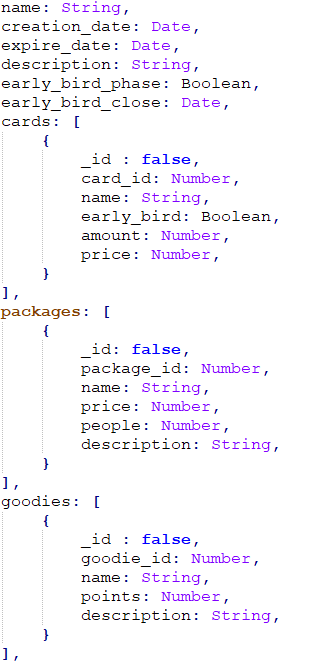
\includegraphics[width=\textwidth,height=\textwidth,keepaspectratio]{events_models.png}
				\caption{Event-Model}
			\end{figure}	
			
			\newpage		
				
			\subsubsection{User}
				\begin{itemize}
					\item 'firstname' der Vorname des User wird vor allem für die Anzeige benutzt
					\item 'lastname' der Nachname des User wird vor allem für die Anzeige benutzt
					\item 'username' der Username des User wird für das ein einloggen verwendet
					\item 'password' das Passwort des Users, welches verschlüsselt abgespeichert wird
					\item 'email' die Email Adresse eines User wird vor allem zum Passwort zurücksetzen verwendet
					\item 'active' eine boolesche Variable, welche angibt ob ein User momentan aktiv seinen Kartenstand verändern kann
					\item 'admin' eine boolesche Variable, welche angibt ob dieser User ein Administrator ist
					\item 'description' eine kurze Beschreibung der Person, die jeder User selbst verändern kann
					\item 'resetkey' der Schlüssel mit dem das Passwort zurückgesetzt wird, wird nur für interne Überprüfungen benutzt
					\item 'request' eine boolesche Variable, welche angibt ob ein User eine Passwortzurücksetzung angefordert hat, wird ebenfalls nur für interne Überprüfungen verwendet
					\item 'events' besteht aus einem Array von Objekten indem alle Events des Users gespeichert werden
					\begin{itemize}
						\item 'event\_id' ist die Identifikation des Events, um welches es sich in diesem Objekt handelt (ObjektId des Events) in einer SQL Architektur würde man dies den Fremdschlüssel nennen
						\item 'active' eine boolesche Variable welche angibt ob dieser User momentan bei diesem Event seinen Kartenstand verändern darf
						\item 'promotion\_start' das Datum an dem dieser User das Event das erste mal zugeteilt wurde, wird für die Statistik verwendet
						\item 'points' der momentane Punktestand des User
						\item 'last\_changed' das Datum an dem der User das letzte mal seinen Kartenstand zu diesem Event aktualisiert hat
						\item 'mone\_submitted' der Betrag, den der User bisher von den verkaufen Karten und Paket abgegeben hat
						\item 'cards' ist ein weiteres Array von Objekten
						\begin{itemize}
							\item 'card\_id' die Identifikationsnummer dieses Kartentyp
							\item 'amount' die Menge an Karten, die ein User von diesem Kartentyp insgesamt bekommen hat
							\item 'sold' die Anzahl an Karten, die der User von diesem Kartentyp verkauft hat
							\item 'submitted' die Anzahl an Karten, die der User von diesem Kartentyp zurückgegeben hat
							\item 'available' die Anzahl an Karten, von diesem Kartentyp welche der User noch im besitzt hat
						\end{itemize}
						\item 'goodies' ist ein weiteres Array von Objekten indem die eingelösten Goodies gespeichert werden
						\begin{itemize}
							\item 'goodie\_id' die Identifikationsnummer dieses Belohnungstyp
							\item 'date\_of\_redeem' das Datum an welchem diese Belohnung das letzte mal verändert wurde
							\item 'amount' Anzahl an Einlösung für diese Belohnung
						\end{itemize}
					\end{itemize}
				\end{itemize}
			\begin{figure}[H]
				\centering
				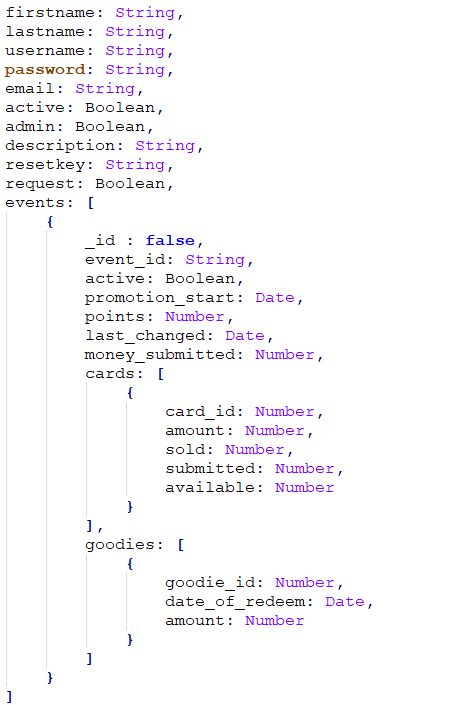
\includegraphics[width=\textwidth,height=\textwidth,keepaspectratio]{user_model.png}
				\caption{User-Model}
			\end{figure}		
		\newpage
		\subsubsection{Entscheidungsgrundlagen}
			Einer der Gründe warum wir uns für die MongoDB entscheiden haben war, dass am Anfang niemand vorhersagen konnte wie genau unsere Datenbank aufgebaut sein wird. 
			Während der Entwicklung gab es viele Informationen, welche nachträglich in die Struktur eingefügt wurden, dies hat uns dieser Anbieter sehr vereinfacht. 
			Ein weiter Grund war die Möglichkeit ein Array aus Objekten zu speichern, was viel Abfragen und logistische Probleme gelöst hat, ins besondere da wir in unserem Backend über die Schnittstelle 'mongoose' auf 
			die Datenbank zugreifen, welche einiges ermöglicht was mit MonogDB alleine nicht realisierbar wäre, wie zum Beispiel das Vorgeben einer Struktur welche aber veränderbar ist und auch ohne Update auf veralte Datensätze immer noch funktioniert. 
			Diese Struktur hat uns auch ermöglicht, dass alle Mitglieder des Teams einen Überblick über die Datenbank bekommen und einfach Abfragen, Updates und Inserts schreiben konnten. 
			Dazu kommt, dass durch die Möglichkeit der Arrays aus Objekten nur zwei Tabellen (Kollektion) benötigt werden, während in einer normalen SQL Datenbank, welche in dritter Normalform ist, mindestens zwölf Tabellen benötigt werden. 
			Natürlich war uns die Performanz der Abfragen sehr wichtig, was ein weiter Grund war warum wir uns für diese Technologie entschieden haben, da die MongoDB eine sehr hohe Performanz hat, selbst beim Abfragen von großen Dokumenten wie sie in unsere Datenbank gespeichert sind. 
			Da die Objekte der MongoDB wie JSON Objekte aufgebaut sind, hat das die Auswertung am Backend ebenfalls erleichtert.

\newpage